\documentclass[usenames,dvipsnames]{beamer}
 
\usepackage[utf8]{inputenc}
\usetheme{Madrid}
\usepackage{setspace}
\usepackage[spanish]{babel}
\usepackage[utf8]{inputenc}
\usepackage{textcomp}
\usepackage{eurosym}
 
 
\title[Trabajo Fin de Grado] %optional
{Aplicación para la planificación y gestión de viajes turísticos}
 
\subtitle{Trabajo Fin de Grado}
 
\author[Rodrigo Dopazo Iglesias]{
\textbf{Autor: Rodrigo Dopazo Iglesias}
\\
\textbf{Director: Juan Raposo Santiago}
}
 
\institute[]
{Grado en Ingeniería Informática\\
Mención en Tecnologías de la Información
\and
Universidade da Coruña\\
Facultad de Informática
}
 
\date
{A Coruña, 2 de Julio de 2018}

\logo{
\includegraphics[height=0.5cm]{./img/logo.png}}


 
\begin{document}

\frame{\titlepage}
 
\begin{frame}
\setlength{\baselineskip}{18pt}
\frametitle{Introducción}
\begin{center}
\textit{¿En qué consiste?\\
¿Qué finalidad tiene?\\
¿A quién está dirigido?\\}
\end{center}
\end{frame}

\begin{frame}
\frametitle{Objetivos}
La realización del proyecto exige la consecución de los siguientes objetivos:
\\
\
\begin{enumerate}
 \item<1-> \textbf{Planificar rutas}
 \item<2-> \textbf{Acceso datos externos}
 \item<3-> \textbf{Gestionar Eventos}
 \item<4-> \textbf{Aplicación móvil y aplicación web}
 \item<5-> \textbf{Datos en tiempo real}
\end{enumerate}
\end{frame}


\begin{frame}
\frametitle{Demo}
\begin{center}

\includegraphics[height=5cm]{./img/video.png}
\end{center}
\end{frame}



\begin{frame}
\frametitle{Índice}
\tableofcontents
\end{frame}



\section{Análisis de Alternativas}
\begin{frame}
\frametitle{Análisis de Alternativas}

\begin{itemize}
 \item Foursquare App
 \item Google Trips: Travel Planner
 \item Sygic Travel
 \item Visit a City
\end{itemize}


\vspace{0.5cm}
\begin{center}

\includegraphics[height=2cm]{./img/FoursquareApp.png}

\includegraphics[height=2cm]{./img/GoogleTrips.png}

\includegraphics[height=2cm]{./img/SygicTravel.png}

\includegraphics[height=2cm]{./img/VisitaCity.png}

\end{center}
\end{frame}



\section{Metodología y Planificación}

\begin{frame}
\frametitle{Metodología y Planificación}
\begin{itemize}
\item Se ha optado por seguir una metodología basada en el \textbf{Proceso Unificado}.
\item \textbf{Iteraciones}:
\begin{itemize}
\item Flujos básicos de trabajo. \textit{Análisis, Diseño, Implementación y Pruebas}.
\item División en tareas.
\item Planificación en tiempo, coste y esfuerzo.
\end{itemize}
\end{itemize}
\end{frame}


\begin{frame}
\frametitle{Metodología y Planificación (II)}
\textbf{Planificación}:


\vspace{0.5cm}
\centering
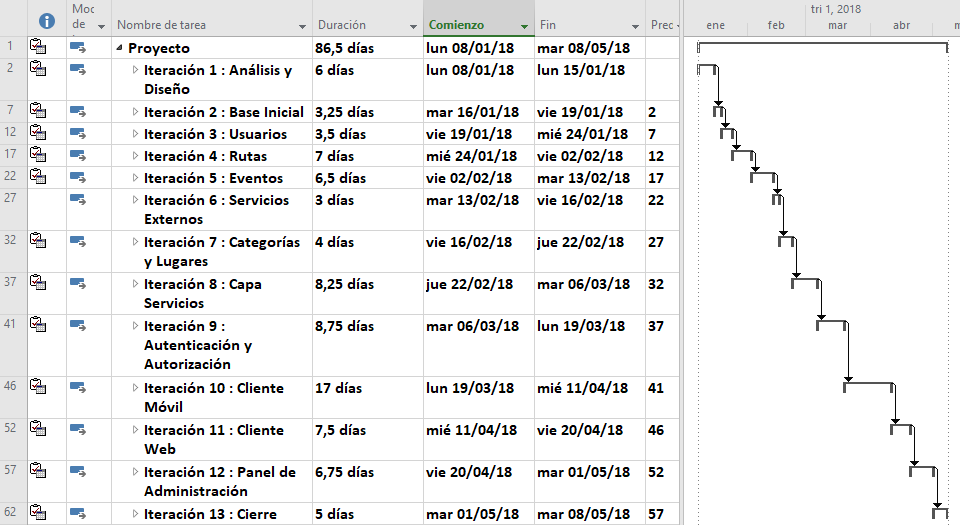
\includegraphics[width=11cm, height=5.8cm]{./img/gantt.png}
\end{frame}


\begin{frame}
\frametitle{Metodología y Planificación (III)}
\textbf{Costes}:
\begin{table}[H]
\centering
\begin{tabular}{|l|c|c|c|}
\hline
\textbf{Recurso} & \textbf{Coste Total} \\ \hline
Recursos Humanos &  10.332 € \\ \hline
Hardware & 1.300 €  \\ \hline
Software & 0 €  \\ \hline
\textbf{Total} & \textbf{11.632 €} \\ \hline
\end{tabular}
\end{table}
\end{frame}



\section{Flujos de Trabajo}
\begin{frame}
\frametitle{Flujos de Trabajo}
\begin{itemize}
\item \textbf{Análisis}:
	\begin{itemize}
		\item Requisitos funcionales y no funcionales.
		\item Actores del sistema.
			\begin{itemize}
				\item Usuario web.
				\item Usuario móvil.
				\item Administrador.
				\item Gestor de eventos.
			\end{itemize}
		\item Diagrama y especificación de casos de uso.
	\end{itemize}
\end{itemize}
\end{frame}

\begin{frame}
\frametitle{Flujos de Trabajo (II)}
\begin{itemize}
\item \textbf{Diseño}:
	\begin{itemize}
		\item Arquitectura en capas.
	\end{itemize}
\end{itemize}

\centering
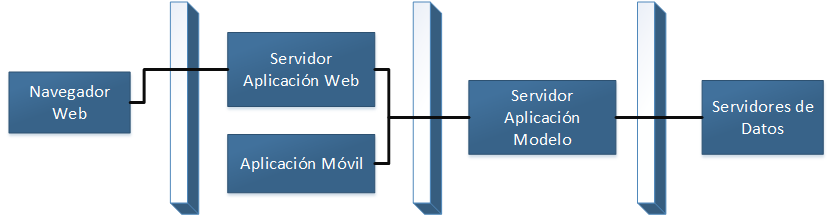
\includegraphics[width=9cm]{./img/arqsistema.png}
\end{frame}

\begin{frame}
\frametitle{Flujos de Trabajo (III)}
\begin{columns}[c] % The "c" option specifies centered vertical alignment while the "t" option is used for top vertical alignment
\column{.5\textwidth} % Right column and width
\centering
\textbf{Arquitectura MVVM}

\column{.5\textwidth} % Left column and width
\centering
\textbf{Arquitectura MVC}
\end{columns}
\vspace{0.3cm}


\centering
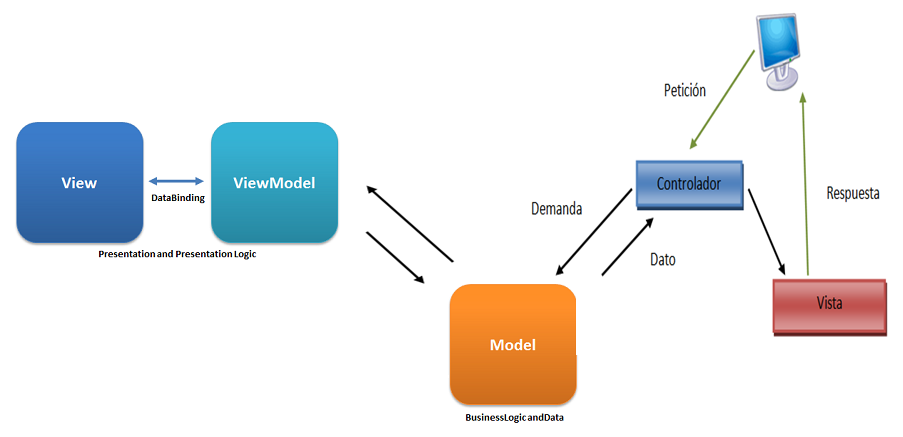
\includegraphics[height=5cm]{./img/MVVM.png}

\end{frame}

\begin{frame}
\frametitle{Flujos de Trabajo (IV)}

\begin{columns}[c] % The "c" option specifies centered vertical alignment while the "t" option is used for top vertical alignment

\column{.4\textwidth} % Left column and width
\textbf{Patrones de diseño:}
\begin{itemize}
	\item DAO
	\item Fachada
	\item DTO
	\item Singleton
	\item Inversión de Control
\end{itemize}

\column{.6\textwidth} % Right column and width
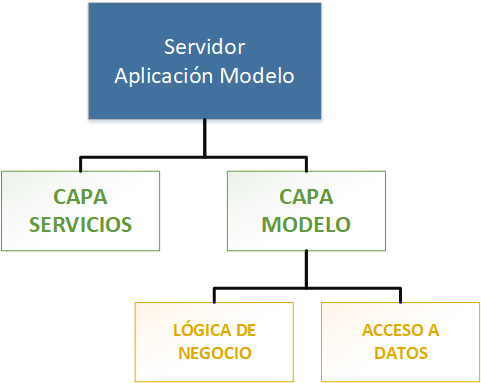
\includegraphics[height=5cm]{./img/arqmodelo.png}

\end{columns}
\end{frame}



\begin{frame}
\frametitle{Flujos de Trabajo (V)}

\begin{itemize}
\item \textbf{Implementación}:
\end{itemize}
\vspace{-0.5cm}
\begin{center}

\includegraphics[height=1.5cm, angle=10]{./img/java.png}

\includegraphics[height=1cm]{./img/maven.png}

\includegraphics[height=1.5cm, angle=8]{./img/spring.png}

\includegraphics[height=1cm, angle=-5]{./img/ionic.png}

\includegraphics[height=1.5cm, angle=-5]{./img/jaxrs.png}

\includegraphics[height=1.5cm, angle=-5]{./img/htmlcssjs.png}

\includegraphics[height=1cm, angle=5]{./img/ajax.png}

\includegraphics[height=0.5cm, angle=5]{./img/thymeleaf.png}


\includegraphics[height=1.5cm, angle=12]{./img/bootstrap.png}

\includegraphics[height=1cm]{./img/oracledb.png}

\includegraphics[height=1.5cm, angle=-5]{./img/tomcat.png}
\end{center}
\end{frame}



\begin{frame}
\frametitle{Flujos de Trabajo (VI)}
\begin{itemize}
\item \textbf{Pruebas}:
	\begin{itemize}
		\item Pruebas de integridad.
		\item Pruebas de sistema.
	\end{itemize}
\end{itemize}

\vspace{0.6cm}
\centering

\includegraphics[height=3cm, angle=0]{./img/testing.png}

\end{frame}

\section{Conclusiones y Líneas Futuras}
\begin{frame}
\frametitle{Conclusiones y Líneas Futuras}
\begin{columns}[c] % The "c" option specifies centered vertical alignment while the "t" option is used for top vertical alignment

\column{.65\textwidth} % Left column and width
\textbf{Conclusiones:}
\vspace{0.4cm}
\begin{itemize}

	\item \textbf{\textcolor{ForestGreen}{Positivas}}
		\begin{itemize}
			\item Cumplimiento de los objetivos.
			\item Conocimiento adquirido.
		\end{itemize}
	\vspace{0.5cm}
	\item \textbf{\textcolor{Red}{Negativas}}
		\begin{itemize}
			\item Dificultades con las nuevas tecnologías.
			\item Fuentes de datos externas.
		\end{itemize}
\end{itemize}

\column{.35\textwidth} % Right column and width
\vspace{-3cm}

\includegraphics[height=2.5cm, angle=0]{./img/conlcusion.jpg}
\end{columns}
\end{frame}


\begin{frame}
\frametitle{Conclusiones y Líneas Futuras (II)}
La aplicación desarrollada supone una base inicial sobre la cual seguir trabajando y mejorando su funcionalidad.
\vspace{0.5cm}
\begin{itemize}

	\item \textbf{A corto plazo:}
		\begin{itemize}
			\item Mejorar interfaz.
			\item Obtención datos de geolocalización.
		\end{itemize}
	\vspace{0.5cm}
	\item \textbf{A largo plazo:}
		\begin{itemize}
			\item Avance hacia red social.
			\item Mejorar sistema gestión de eventos.
			\item Incorporar más funcionalidades de personalización.
		\end{itemize}
\end{itemize}
\end{frame}
 
 

\begin{frame}
\centering
\institute[]{
\alert{\Large{Gracias por su atención}}}
\maketitle


\end{frame}
                
                  
\end{document}